\chapter{Additional Plots}

\begin{figure}[H]
    \centering
    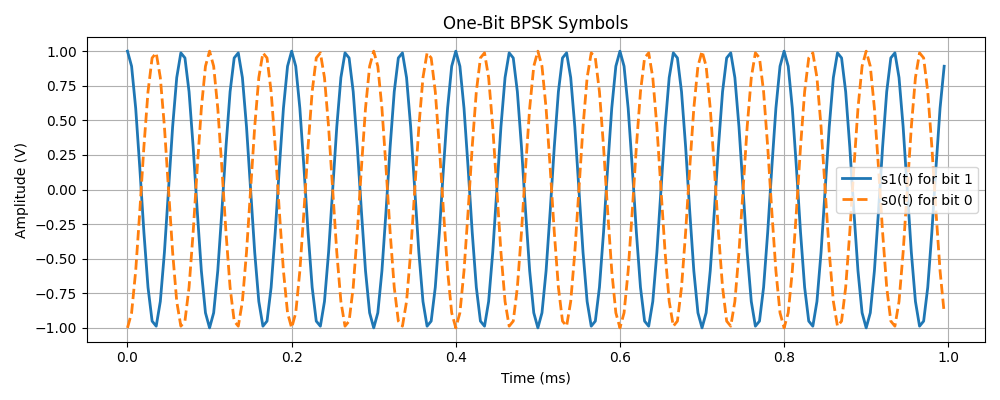
\includegraphics[width=0.85\textwidth]{plots/bpsk.png}
    \caption{BPSK symbols for bits 1 and 0}
\end{figure}

\begin{figure}[H]
    \centering
    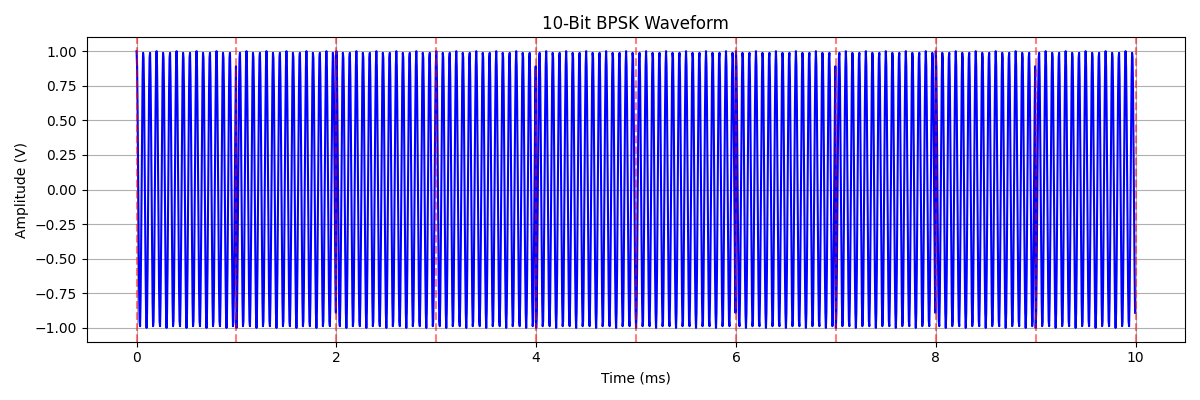
\includegraphics[width=0.85\textwidth]{plots/10-bit_wave.png}
    \caption{10-bit BPSK waveform with bit boundaries}
\end{figure}

\begin{figure}[H]
    \centering
    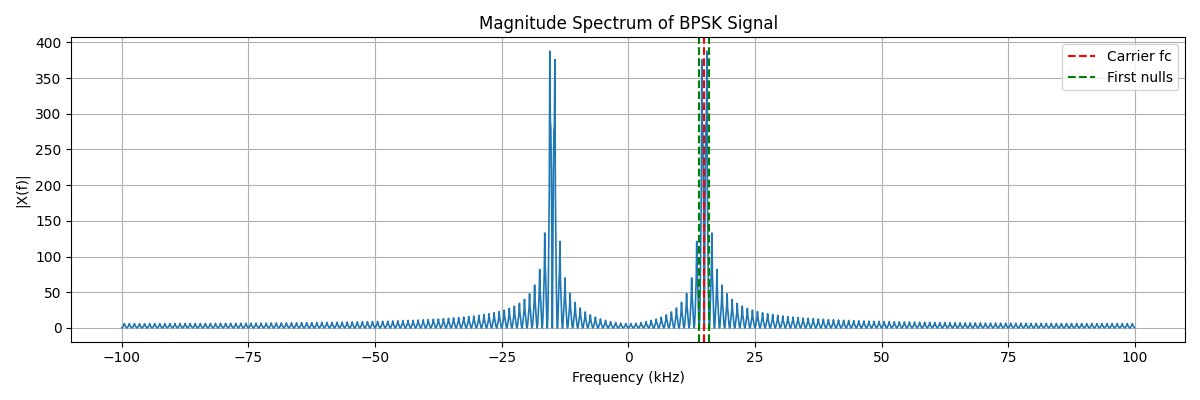
\includegraphics[width=0.85\textwidth]{plots/magnitude_spectrum_of_bpsk.png}
    \caption{FFT magnitude spectrum of the BPSK waveform}
\end{figure}

\begin{figure}[H]
    \centering
    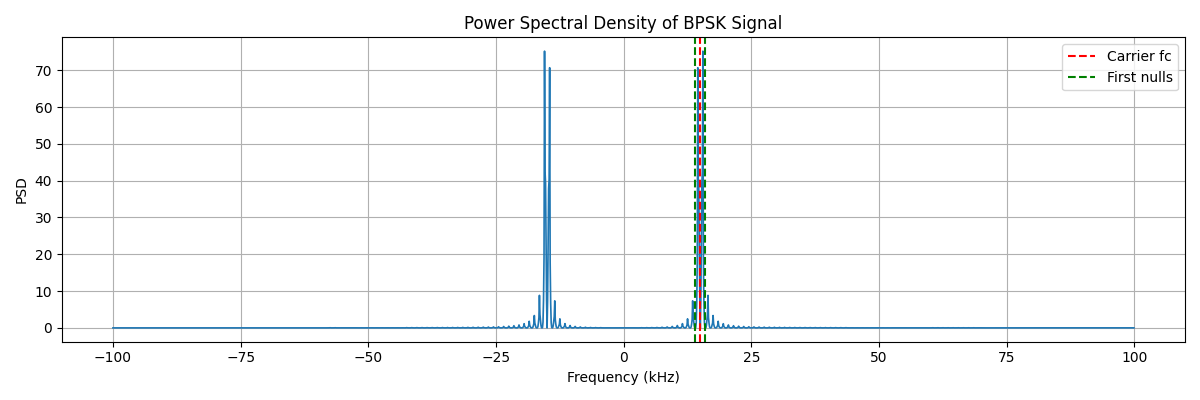
\includegraphics[width=0.85\textwidth]{plots/power_spectral_density_bpsk.png}
    \caption{Power spectral density of the BPSK waveform}
\end{figure}

\begin{figure}[H]
    \centering
    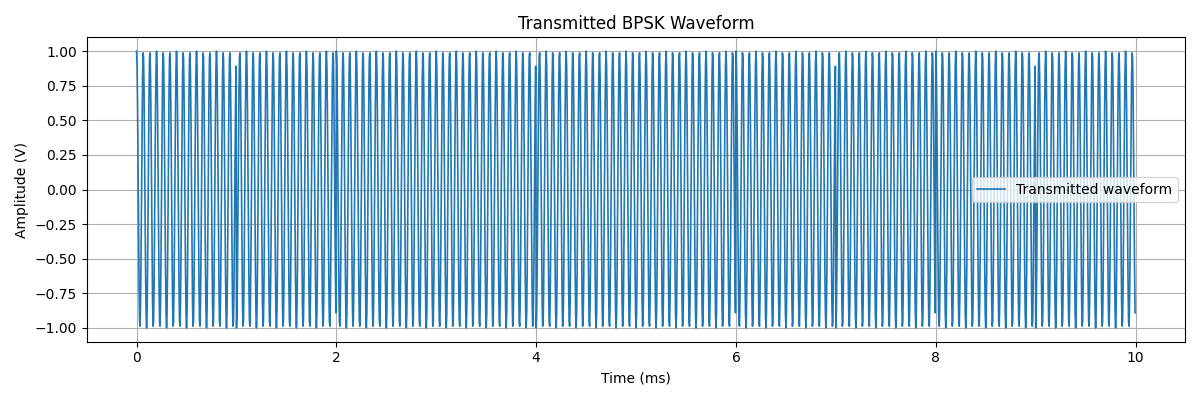
\includegraphics[width=0.85\textwidth]{plots/transmitted_bpsk.png}
    \caption{Transmitted signal through mild low-pass channel}
\end{figure}

\begin{figure}[H]
    \centering
    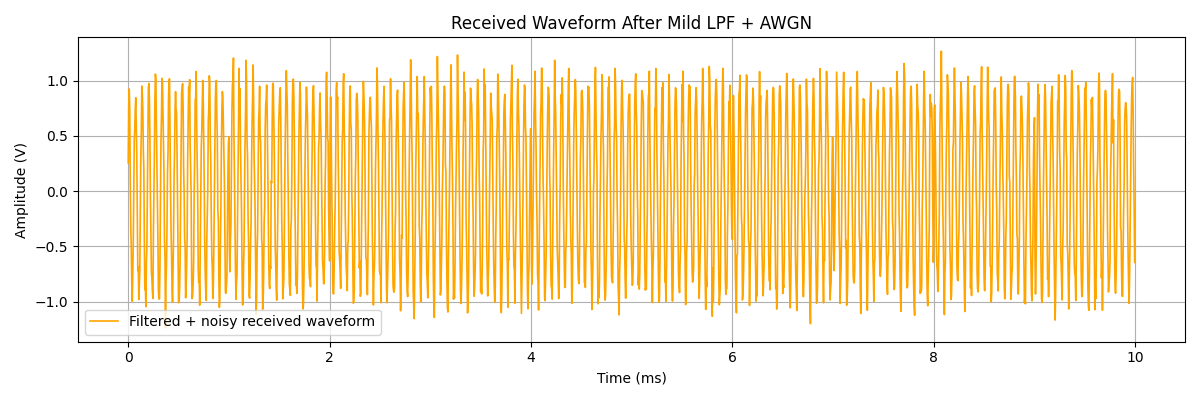
\includegraphics[width=0.85\textwidth]{plots/received_wave.png}
    \caption{Received waveform after channel and noise}
\end{figure}

\begin{figure}[H]
    \centering
    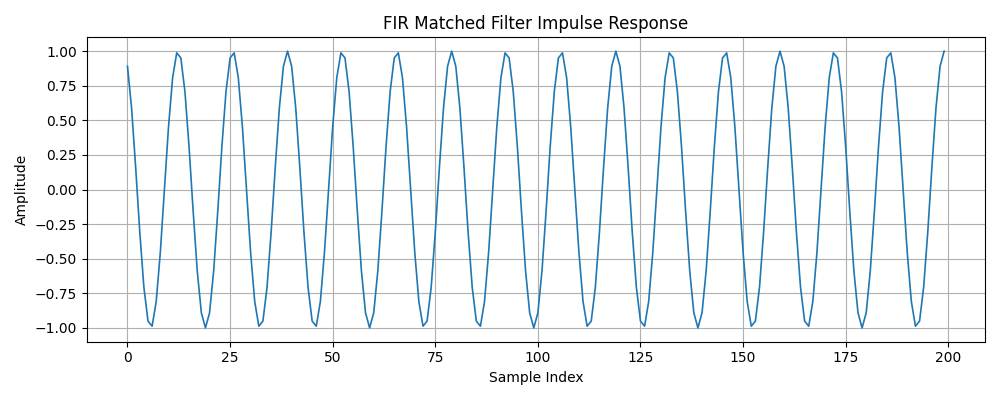
\includegraphics[width=0.85\textwidth]{plots/fir_impulse_response.png}
    \caption{FIR matched filter impulse response}
\end{figure}

\begin{figure}[H]
    \centering
    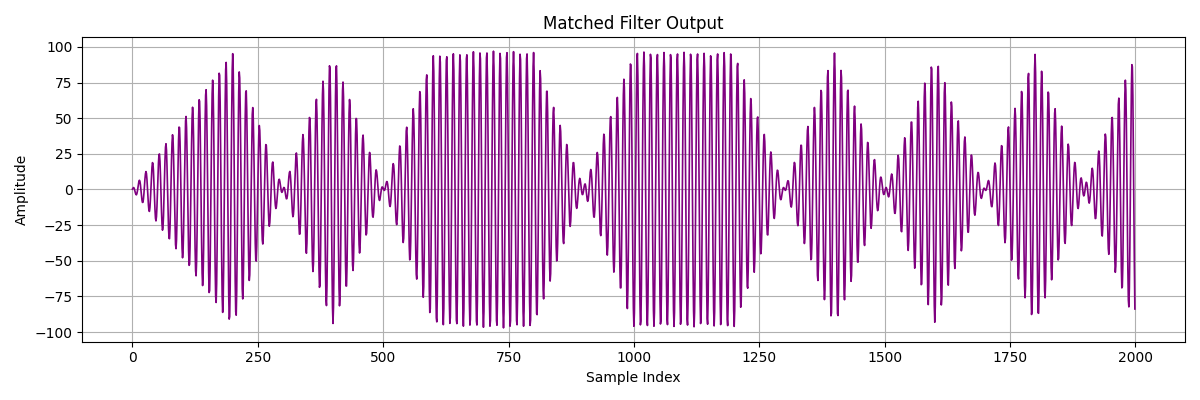
\includegraphics[width=0.85\textwidth]{plots/matched_filter_output.png}
    \caption{Matched filter output}
\end{figure}

\begin{figure}[H]
    \centering
    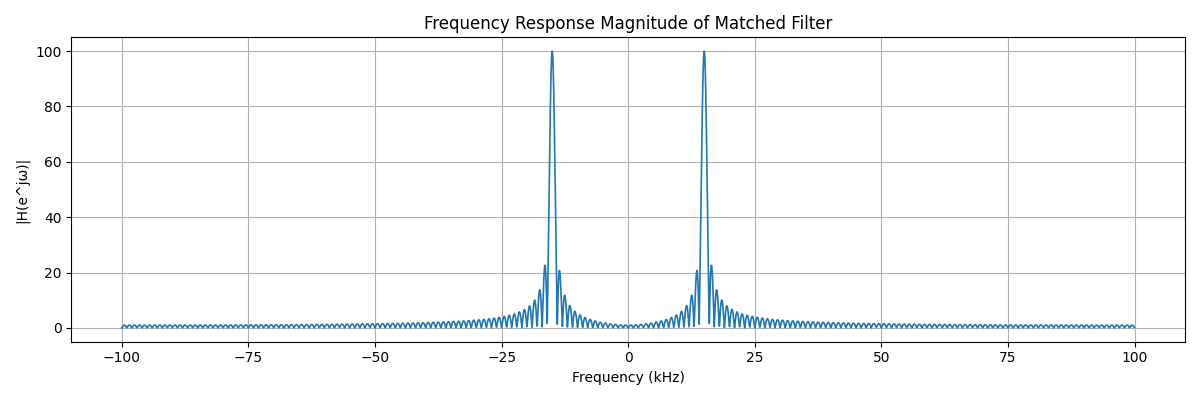
\includegraphics[width=0.85\textwidth]{plots/frequency_response_matched_filter.png}
    \caption{Frequency response of the FIR matched filter}
\end{figure}

\begin{figure}[H]
    \centering
    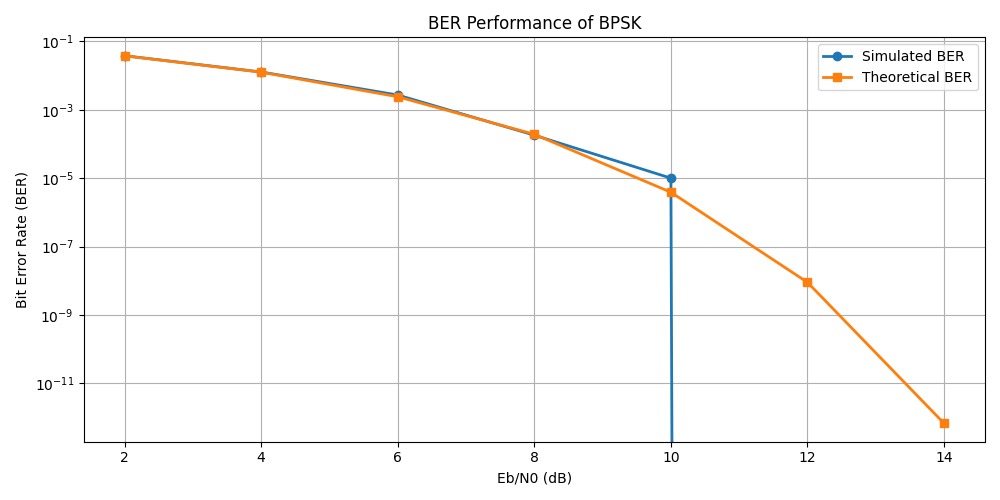
\includegraphics[width=0.85\textwidth]{plots/ber.png}
    \caption{Simulated and theoretical BER comparison}
\end{figure}

\begin{figure}[H]
    \centering
    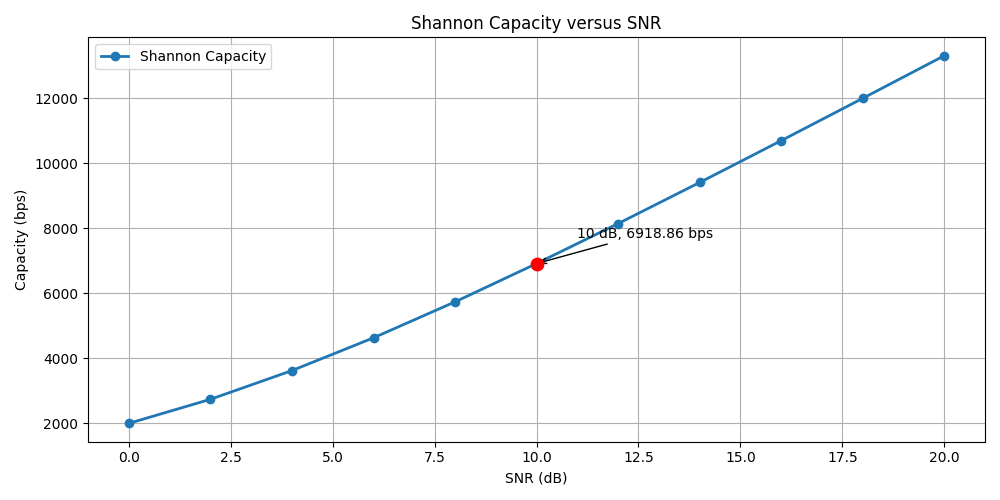
\includegraphics[width=0.85\textwidth]{plots/shannon_capacity_vs_snr.png}
    \caption{Shannon capacity versus SNR}
\end{figure}